
\chapter{Budowa prototypu}

Prezentowany prototyp składa się z dwóch części: nadajnika i odbiornika, pomiędzy którymi
dokonywany jest pomiar odległości. W niniejszym rozdziale przedstawiono zasadę funkcjonowanie 
poszczególnych komponentów.

\section{Budowa i zasada działania nadajnika}

Nadajnik zbudowany został na bazie płytki prototypowej \textit{Arduino Nano} \cite{bib:arduinoNano},
która składa się z procesora ATmega328 \cite{bib:atmega328} taktowanego rezonatorem kwarcowym \SI{16}{MHz},
stabilizatora napięcia \SI{5}{V} oraz układu FT232RL umożliwiającego 
jej programowanie  ze środowiska \textit{Arduino} \cite{bib:Arduino} za pośrednictwem portu USB. 
\textit{Arduino Nano} połączono 
bezpośrednio z czterema nadajnikami ultradźwiękowymi (głośnikami, rezonatorami piezoelektrycznymi) typu 40ST-12 \cite{bib:40ST12}.
Do płytki doprowadzono zasilanie oraz sygnały sterujące z odbiornika złączem SV1. 
Schemat połączeń przedstawia rysunek \ref{fig:nadajnik_schemat}.

 \begin{figure}[h]
    \centering
    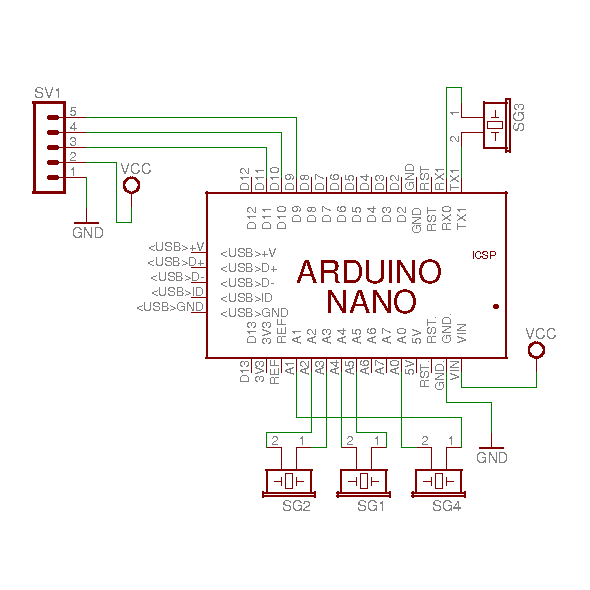
\includegraphics[width=0.6\textwidth, trim= 0mm 0mm 0mm 0mm,clip]{transmitter}
    \caption{Schemat nadajnika}
    \label{fig:nadajnik_schemat}
\end{figure}

Całość umieszczono na ramie w kształcie litery H wykonanej z rurek PCV.
Rezonatory dodatkowo odizolowano  od ramy przy użyciu rzepów, co ułatwia ich demontaż, a także skutecznie
zapobiega przenoszeniu się drgań. 

\rysunek{nadajnik_H}{Szkic ramy nadajnika}{\label{fig:nadajnik_szkic}}


\textit{Android Nano} połączony jest z odbiornikiem sześciometrowym kablem, którym przesyłane są sygnały sterujące oraz zasilanie.
Do sterowania wykorzystywano trzy przewody -- dwa z nich informują, który z głośników ma w danym momencie nadawać,
a trzeci służy jako wyzwalacz. 
Informacja, który z głośników  ma nadawać kodowana jest za pomocą dwóch bitów w systemie binarnym,
napięcie na przewodzie \SI{3,3}{V} oznacza logiczną jedynkę, a \SI{0}{V} oznacza logiczne zero.

Na potrzeby nadajnika powstało oprogramowanie w C dla procesora ATmega328 generujące nadawany sygnał.
Cała logika programu mieści się w obsłudze przerwania sprzętowego, które reaguje na opadające zbocze na wyzwalaczu.
Gdy wyzwalane jest przerwanie, oprogramowanie wysyła z góry zdefiniowany sygnał do odpowiedniego rezonatora. 
Nadawany sygnał jest tak dobrany, by dało się go w prosty sposób wyodrębnić. Składa się z dwóch
części: wzbudzającej oraz tłumiącej.
Okres impulsów sygnału jest zgodny z częstotliwością rezonansową przetworników, a dodatkowo część tłumiąca
jest przesunięta względem części wyzwalającej o 180 stopni.  
Rysunek \ref{fig:output_signal} przedstawia sygnał, jaki podawany jest na przetwornik piezoelektryczny.

\begin{figure}[h]
    \centering
    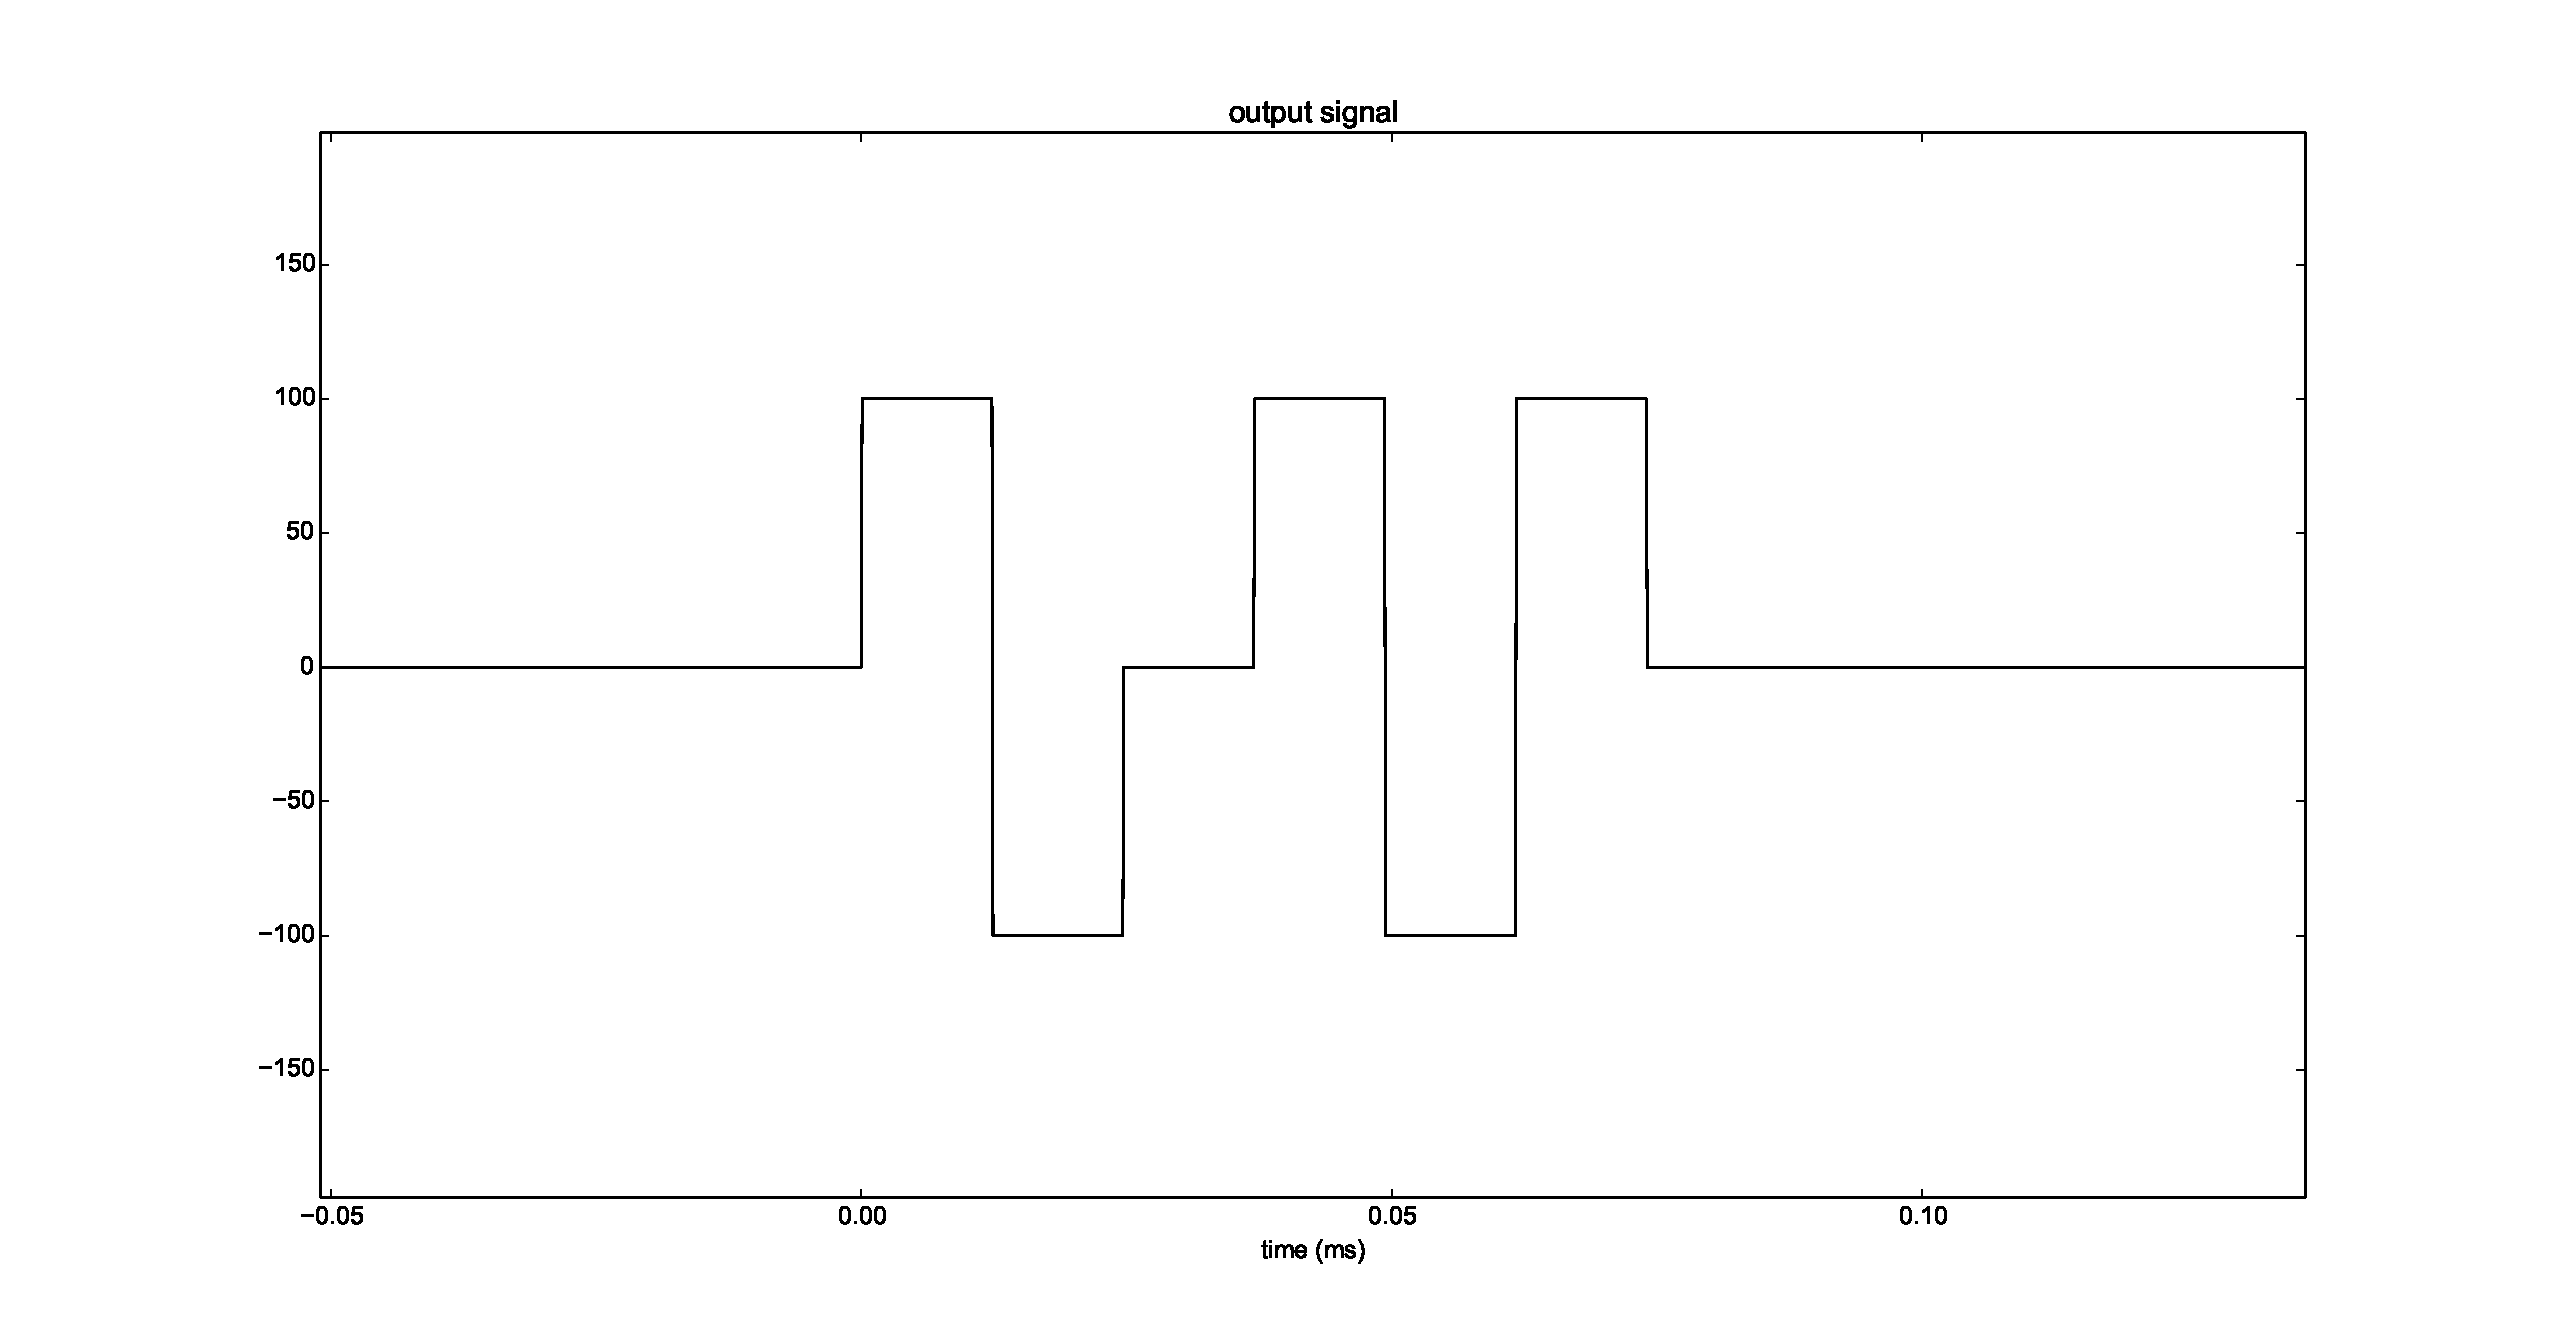
\includegraphics[width=1.15\textwidth, trim= 47mm 0mm 0mm 0mm,clip]{output_signal}
    \caption{Sygnał podawany na przetwornik piezoelektryczny}
    \label{fig:output_signal}
\end{figure}

\section{Dobór rezonatorów piezoelektrycznych}

Głównym problemem podczas konstrukcji nadajnika okazał się dobór odpowiednich rezonatorów piezoelektrycznych.
Mimo że producent wykorzystanych rezonatorów zapewnia ich pracę w zakresie \SI{40}{kHz} $\pm$ \SI{1}{kHz},
to taki rozrzut okazał się zbyt duży, 
dlatego z 30 rezonatorów (15 nadajników i 15 odbiorników) wybrane zostały 4 nadajniki i 3 odbiorniki o najbardziej 
zbliżonych częstotliwościach rezonansowych.

Tabela \ref{table:czestotliwosci} zawiera wyniki pomiarów częstotliwości. Gwiazdką oznaczono wykorzystane przetworniki piezoelektryczne.

\begin{table}[t]
  \caption{Częstotliwości rezonansowe przetworników piezoelektrycznych}
  \label{table:czestotliwosci}
  \centering
  \begin{tabular}{|r|r|r|}
    \hline 
    Nr & Nadajnik 40ST-12 & Odbiornik 40SR-12\\
    \hline
    1  &   \SI{40,88}{kHz} & *\SI{40,65}{kHz} \\
    2  &   \SI{41,12}{kHz} &  \SI{40,45}{kHz} \\
    3  &  *\SI{40,78}{kHz} &  \SI{39,52}{kHz} \\
    4  &   \SI{41,19}{kHz} &  \SI{40,47}{kHz} \\
    5  &   \SI{40,92}{kHz} &  \SI{40,66}{kHz} \\
    6  &   \SI{39,68}{kHz} & *\SI{40,69}{kHz} \\
    7  &   \SI{39,78}{kHz} &  \SI{40,59}{kHz} \\
    8  &  *\SI{40,80}{kHz} &  \SI{40,39}{kHz} \\
    9  &   \SI{40,90}{kHz} &  \SI{40,29}{kHz} \\
    10 &  *\SI{40,66}{kHz} & *\SI{40,68}{kHz} \\
    11 &  *\SI{40,85}{kHz} &  \SI{39,22}{kHz} \\
    12 &   \SI{41,01}{kHz} &  \SI{39,51}{kHz} \\
    13 &   \SI{41,00}{kHz} &  \SI{39,92}{kHz} \\
    14 &   \SI{39,82}{kHz} &  \SI{39,26}{kHz} \\
    15 &   \SI{39,64}{kHz} &  \SI{39,11}{kHz} \\
    \hline
  \end{tabular}
\end{table}


